This sections describes the simulation interaction between agents. Of the
research directions presented in this chapter, it is definitely the most
malleable. Deciding how a simulation is structured from an interactions
standpoint is a delicate balance of known necessity and perceived future
needs. There are basic decisions to make: do you want a system with discrete
material transfers or continuous material flows? Discrete transfers more closely
match reality and may provide insights in that regard, however the require more
of their modeling apparatus due to messaging needs and other structures. More
complex decisions include how one wants to determine connections between
facilities. Do we assign supplier-consumer pairs to facilities? Do we allow them
to change? Should the facility make such a decision? Should that decision be
affected by any other entities? Guerin's comment in \S\ref{sec:intro-benchmarks}
stems from this ``freedom''. These simulation-engine decisions comprise the
art-related portion of fuel cycle simulation. The goal is to make these
decisions in as informed a way as possible from our domain-level knowledge with
respect to our known and perceived requirements. In general, we try to minimize
the sheer number of choices we make in this regard, instead relying on well
known and well documented practices of computer scientists and systems
engineers.

\Cyclus has an additional goal in that we wish our core simulation
infrastructure to be as flexible as possible. Given a few basic tenets of agent
interaction, other developers should be able to create a new agent to ``plug
in'' to the simulation. Accordingly, we must define a minimal set of behaviors
to sufficiently inform the simulation infrastructure to run the simulation. This
freedom allows us to run the simulation program and attach agents at run time,
effectively separating the simulation engine's functionality from the agents in
the simulation. From an ecosystem point of view, being an open source code and
having such capability allows expansion of the user and developer base into
areas and institutions concerned with security and privacy. Furthermore,
developers could participate both privately and publicly, e.g. adding general
capability to the \Cyclus core that is needed for some functionality without
specifying the internals. Such a community paradigm is shown in Figure
\ref{fig:community}.

\begin{figure}[htbp!]
  \begin{center}
    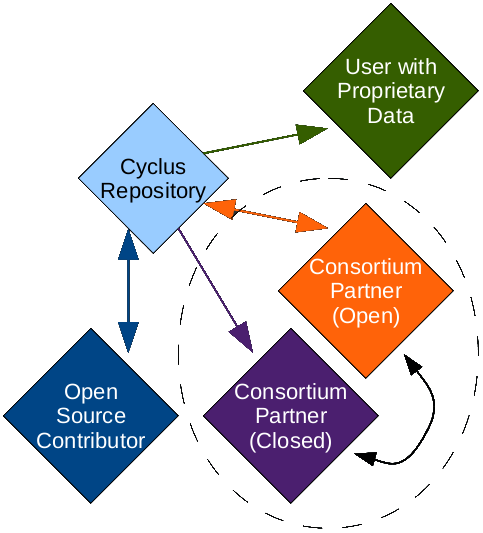
\includegraphics[height=8cm]{./parts/research/community.png}
  \end{center}
  \caption{The Cyclus Participation Paradigm} 
  \label{fig:community}
\end{figure}

This open-source ecosystem further provides incentive to develop the agent-based
simulation architecture. Other developers can concentrate their efforts on
individual agent interaction, effectively encapsulating developer requirements
for learning and interacting with the various simulation systems. Having decided
upon agent-based interactions, one must determine a way to govern these
interactions. We want to minimize agent dependency due to our above discussion,
so using preference-based network flow formulations provide us with a viable
solution technique that provides a consistent interface. The remainder of this
section describes how that market resolution interface is informed by the
agents. Basic agent simulation interaction, such as entering and leaving the
simulation are also described.

\subsection{Supply/Demand Parameters}

The resolution of supply and demand at any given time step is the result of the
mathematical program techniques described in \S\ref{sec:gfctp}; however, there
are simulation-engine details that must be described in order to set up that
problem. The proposed resolution mechanism occurs in nominally three steps. The
agent interactions include consumers and producers of a set of commodities and
progresses is steps or ``phases''. The terminology of this ``phase space'' is
taken from previous supply chain agent-based modeling
work \cite{julka_agent-based_2002}.

The first phase allows consumers of commodities to denote both the quantity of a
commodity they need to consume as well as the target isotopics, or
quality. Because the action of posting is technically telling possible providers
what type of product or service is required by a facility, this phase is termed
the ``Request for Bids Phase''. This action is considered a ``posting'' of
demand to the market exchange. Consumers are allowed to ``over-post'', i.e.,
request more quantity than they can actually consume as long as a corresponding
capacity constraint accompanies this posting. Further, consumers are allowed to
post demand for multiple commodities that may serve to meet the same combine
capacity. For example, consider an LWR that can be filled with MOX or UOX. It
can post a demand for both, but must define a preference over the set of
possible commodities it can consume. Another example is that of an advanced fuel
fabrication facility, i.e., one that fabricates fuel partially from separated
material that has already passed through a reactor. Such a facility can choose
to fill the remaining space in a certain assembly with various types of fertile
material, including depleted uranium from enrichment or reprocessed uranium from
separations. Accordingly, it could demand both commodities as long as it
provides a corresponding constraint with respect to total consumption. At the
end of the posting phase, the market exchange will have a set of consumption
portfolio for each consumer. Each consumption portfolio may be constituted by
multiple consumption requests, and each may have a detailed isotopic quality
defined; however, there must be a cardinal preference over the requests in the
portfolio and an overall capacity for the portfolio.

The second phase allows suppliers to ``respond'' to the set of consumption
portfolios. Each portfolio is comprised of requests for some set of
commodities. Accordingly, for each request, suppliers of that commodity denote
production capacities and an isotopic profile of the commodity they can
provide. This isotopic profile is part of a heuristic mechanism to assign more
fine-grained preferences among suppliers and consumers. Suppliers are allowed to
offer the null set of isotopics as their profile, effectively providing no
information. A supplier may have its production be constrained by more than one
parameter. For example, a processing facility may have both a throughput
constraint (i.e., it can only process material at a certain rate) and an
inventory constraint (i.e., it can only hold some total material). Further, the
facility could have a constraint on the quality of material to be processed,
e.g., it may be able to handle a maximum radiotoxicity for any given time step
which is a function of both the quantity of material is processes but also the
isotopic content of that material. The formulation provided in \S\ref{sec:gfctp}
allows for multiple of such constraints as long as they are linear functions of
the demanded commodity quantity. This phase is termed the ``Response to Request
for Bids Phase'', and at its completion the possible connections between supplier and
producer facilities, i.e., the arcs in the graph of it transportation problem,
have been established with specific capacity constraints defined both by the
quantity of commodities that will traverse the arcs but also by the quality.

The third phase of setting the exchange market parameters involves setting
preference values for each supplier-consumer arc, thus this phase is termed the
``Preference Assignment Phase''. These values will eventually be converted to
costs in order to solve variant of the multi-commodity transportation problem,
in which the inversion technique itself is a simulation design decision. In any
case, this phase begins with the consumers. Each consumer has already assigned
preferences as a function of commodity amongst requests in its portfolio. The
consumer is now allowed to inform the solver as to preferences amongst the
responses to each request in each portfolio. These delineations will nominally
be made as a function of the quality of the material in the big response. For
example, a reactor may request MOX and UOX. It may get two responses to its
request for MOX, each with different isotopic profiles of the MOX that can be
provided. It can then assign preference values over this set of potential MOX
providers. Another prime example is in the case of repositories. A repository
may have a defined preference of material to accept based upon its heat load or
radiotoxicity, both of which are functions of the quality, or isotopics, of a
material. In certain simulators, limits on fuel entering a repository are
imposed based upon the amount of time that has elapsed since the fuel has exited
a reactor. It is in this phase that the \Cyclus engine would allow such
capability. The time constraint is, in actuality, a constraint on heat load or
radiotoxicity (one must let enough of the fission products decay). A repository
could analyze possible input fuel isotopics and set the arc preference of any
that violate a given rule to 0, effectively eliminating that arc. Once
facilities have completed their preference assignments, their managers are able
to permute them based on institutional or regional factors, explained below.

\subsection{Facilities}

Facilities in \Cyclus are abstracted to either consumers or suppliers of
commodities, and some may be both. Supplier agents are provided agency by being
able to communicate to the market-resolution mechanism a variety of production
capacity constraints in phase two of the solution setup. Consumer agents are
provided agency by being able to assign preferences among possible suppliers
based on the supplier's quality of product. Because this agency is encapsulated
for each agent, it is possible to define strategies that can be attached or
detached to the agents at run-time. Such strategies are an example of the
Strategy design pattern \cite{vlissides_design_1995}.

\subsection{Institutions}

Institutions in \Cyclus manage a set of facilities. They are tasked with the
actual instantiation of specific facilities, e.g. it is the institutions job to
manage which facilities are commissioned and decommissioned at the appropriate
times. The goal of including a notion of institutions is to allow an increased
level of detail when investigating regional-specific scenarios. For example,
there exist multi-national enterprises, such as AREVA, that operate fuel cycle
facilities in a variety of countries, or regions. Furthermore, there are
international governmental organizations, such as the IAEA, which operate fuel
cycle facilities that service other facilities in a variety of regions. A fuel
bank is an example of such a facility. Accordingly, institutions in \Cyclus are
able to augment the preferences of supplier-consumer pairs that have been
established in order to simulate a mutual preference to trade material within an
institution. Of course, situations arise in real life where an institution has
the capability to service its own facilities, but choose to use an outside
provider because of either cost or time constraints. Such a situation is allowed
in this framework as well. It is not clear how such a relationship should be
instantiated and to what degree institutions should be allowed to affect their
managed facilities' preferences. This issue lies squarely in the realm of
simulation design decisions, part of the ``art'' of simulation. Accordingly,
through the course of research, the possible design space will be analyzed in
order to determine best practices for this type of design.

\subsection{Regions}

Regions in \Cyclus are concerned with meeting certain requirements, e.g. power
capacity, fuel cycle service capacity, etc. The notion of which facilities will
meet this capacity is abstracted away from the region into the set of
institutions that operate in that region. In other words, in the case of nuclear
power capacity, a region knows that it needs additional reactors to be built,
but leaves the building of those reactors to the institutions that operate in
the region. However, given information regarding the possible reactors that can
be built, the region can order which reactors should be built by which
institutions. Again, the idea here is to abstract the management of facilities
away from the decision of which facilities to build. It is important to note
here that this abstraction allows for different deployment algorithms to be
tested and exchanged in the \Cyclus framework without necessitating changes to
the simulation engine, as is the case with other simulators described
in \S\ref{sec:simulators} and is consistent with the types of simulation design
decisions described in \S\ref{sec:simulators-overview}. Regions are further
provided agency by their ability to affect preferences between supplier-consumer
facility pairs in the third phase of the market resolution algorithm. The
ability to perturb arc preferences between a given supplier and a given consumer
allows fuel cycle simulation developers to model relatively complex interactions
at a regional level. Examples of such interactions include the notion of
tariffs, i.e., a region may prefer that facilities that can trade within its
borders to so. Further, one could model the affect of sanctions, i.e., a region
may not allow trade between facilities within its borders and another specified
region. Finally, constraints can be applied on the quality of material that may
occur in a transaction. For example, a region could scan the set of possible
material leaving its borders via supplier transactions. It could then affect the
preference of transactions that violate some principle, such as ``no MOX can
leave my boundaries''. These principles can even exist on a spectrum, e.g. ``no
MOX with a certain content can leave my boundaries'', or be region-specific,
e.g. ``no MOX can leave my boundaries that will go to some specified
region''. Again, these policies are prime examples of strategies that can be
implemented via the Strategy pattern.
